\section{\ce{[Zn(SCN)_2(4-hydroxymethylpyridine)_2]}}
\subsection{Synthesis}
0.13 g \ce{ZnCl_2} (1 mmol), 0.19 g KSCN (2 mmol) and 0,22 g 4-OH-Me-py (2 mmol) were dissolved in 15 mL distilled \ce{H_2O}. The solution was heated up to 50-60$^\circ$C  and stirred for 1 hour. After filtration the clear solution was stirred again for 1 hour (50$^\circ$C) and then cooled down to RT. After 24 hours clear white crystals were obtained. Anal. Calculated for \ce{C_{14}H_{14}N_{4}O_{2}S_{2}Zn} (399.80 g/mol) : 42.06\% C; 3.53\% H; 14.01\% N; 16.04 \% S; Found: 41.84 \% C; 3.54\% H; 14.00 \% N; 15.89\% S; IR (ATR, cm$^{-1}$): 3409 (s), 2075 (s), 1621 (s), 1562 (w), 1508 (vw), 1452 (w), 1429 (m), 1340 (w), 1277 (w), 1224 (m), 1105 (w), 1034 (s), 949 (w), 807 (m), 722 (w), 657 (vw), 607 (m), 472 (s)

\begin{figure}[h!]
\centering
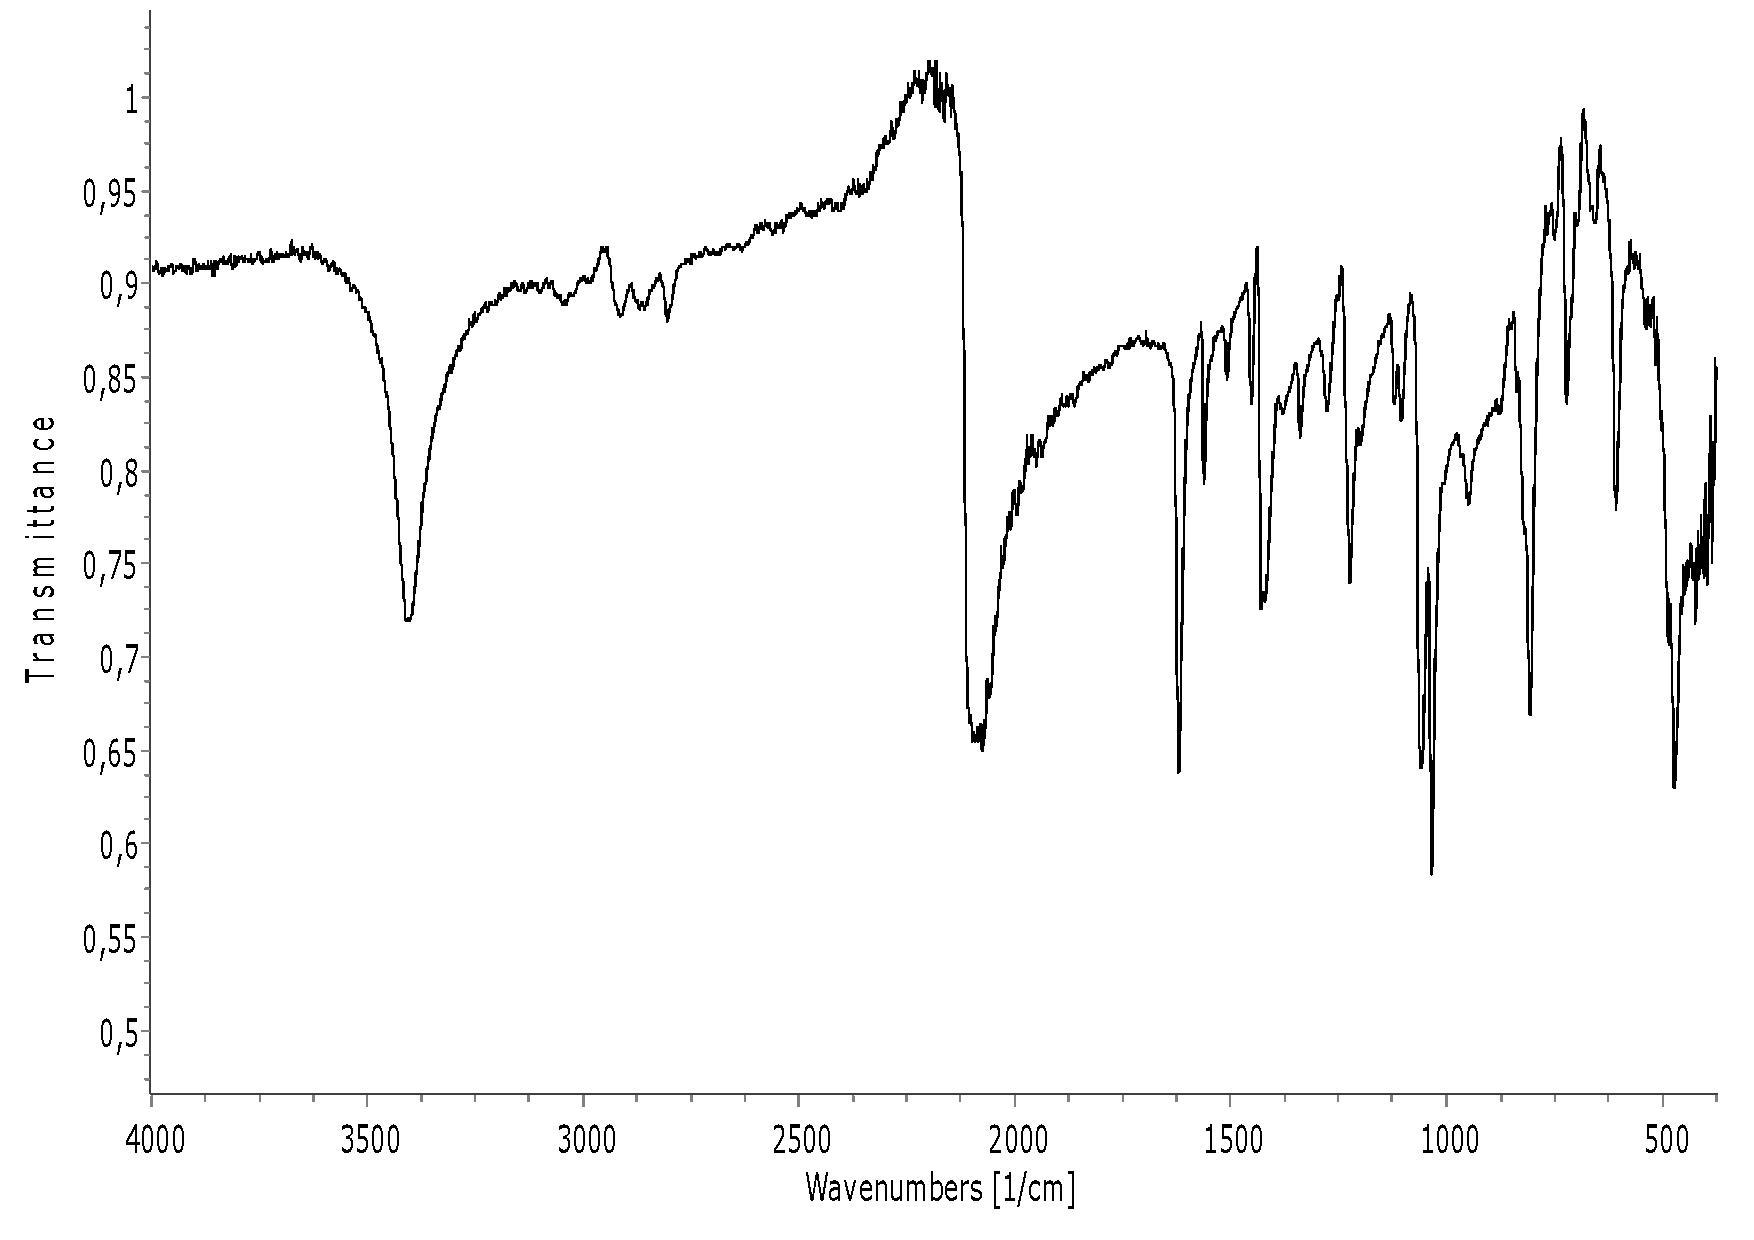
\includegraphics[scale=0.5, width=1\textwidth]{figures/ZnR4HOMP-IR.pdf}
\caption{IR spectrum of \ce{[Zn(SCN)_2(4-HOMepy)_2]}}
\end{figure}

\newpage
\subsection{Structural characterization}

The crystal structure of \ce{[Zn(SCN)_2(4-HOMepy)_2]} consists of two crystallographically independent mononuclear and neutral Zn(II) complexes. A  packing view is shown in fig. \ref{fig:ZnR4HOMP_pv}, a perspective view in fig. \ref{fig:ZnR4HOMP_pv} and selected bond parameters are listed in table \ref{batab:ZnR4HOMP}. Each Zn(1) is tetrahedrally coordinated by N atoms of two terminal isothiocyanato anions, and by N atoms of two neutral 4-hydroxymethylpyridine molecules. The Zn-N bond distances range from 1.939(2) to 2.019(2) \AA, and the bond angles within the \ce{ZnN4} tetrahedron vary from 103.81(9) to 124.28(15)$^\circ$. The bond parameters of terminal N-coordinated NCS- anions are: Zn-N-C = 169.0(2) and 174.3(2)$^\circ$, N-C-S = 177.8(3) and 177.6(3)$^\circ$, N-C = 1.159(4) and 1.158(4) \AA, C-S = 1.627(3) and 1.627(3) \AA.The shortest metal-metal separation is 5.0296(9) \AA. Hydrogen bonds of type O-H\ce{***}S form a supramolecular 2D system [O(1)-H(91)\ce{***}S(2\#1)(\#1: x,2-y,1/2+z) = 165(5)$^\circ$, O(1)\ce{***}S(2\#1) = 3.238(3) \AA; O(2)-H(92)\ce{***}S(1\#2)(\#2: x,-1-y,-1/2+z) = 162(3)$^\circ$, O(1)\ce{***}S(2\#1) = 3.263(3) \AA].




\begin{table}[htpb!]
\centering
\captionabove{Selected bond lengths (\AA) and angles ($^\circ$) for \ce{[Zn(SCN)_2(4-HOMepy)_2]}; Symmetry codes: (‘): -x,y,-z+1/2; (“): 1-x,y,-z+1/2}
\begin{tabular}{|l|l|l|l|}
\hline
Zn(1)-N(1') & 1.939(2) & Zn(2)-N(2'') & 1.943(2)\\
\hline
Zn(1)-N(3) & 2.019(2) & Zn(2)-(N(4) & 2.018(2)\\
\hline
N(1)-C(1) & 1.159(4)& S(1)-C(1) & 1.627(3)\\
\hline
N(2)-C(2) & 1.158(4) & S(2)-C(2) & 1.627(3)\\
\hline
\hline
N(1)-Zn(1)-N(1') & 124.28(15) & N(2)-Zn(2)-N(2'') & 121.03(15)\\
\hline
N(1')-Zn(1)-N(3) & 105.90(10) & N(2'')-Zn(2)-N(4) & 103.53(9)\\
\hline
N(1')-Zn(1)-N(3') & 105.23(9) & N(2'')-Zn(2)-N(4'') & 108.81(9)\\
\hline
Zn(1)-N(11)-N(12) & 109.92(13) & N(4)-Zn(2)-N(4'') & 111.17(13)\\
\hline
Zn(1)-N(1)-C(1) & 169.0(2) & N(1)-C(1)-S(1) & 177.8(3)\\
\hline
Zn(2)-N(2)-C(2) & 174.3(2) & N(21)-C(2)-S(2) & 177.6(3)\\
\hline
\end{tabular}

\label{batab:ZnR4HOMP}
\end{table}




\begin{figure}[!htpb]
\centering
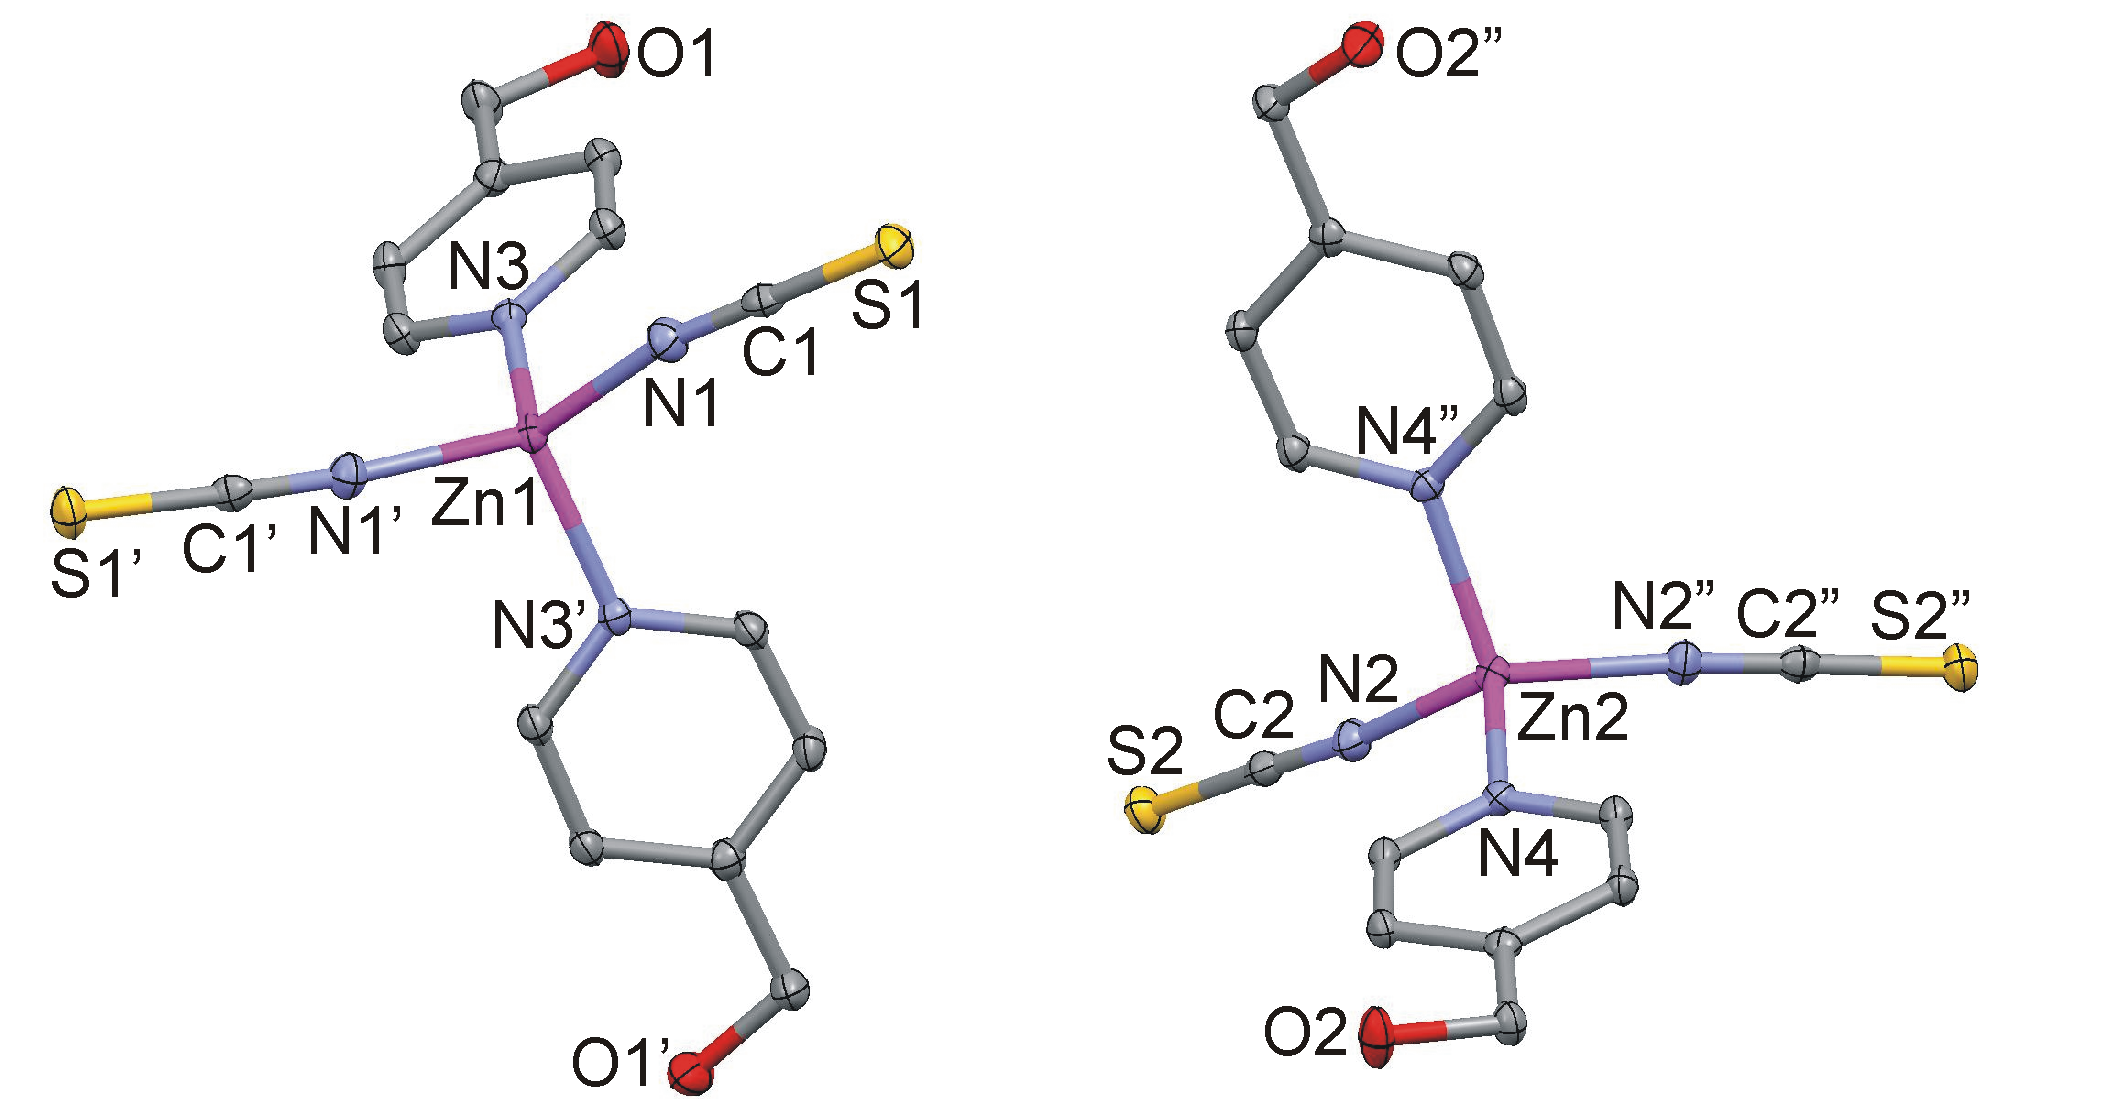
\includegraphics[width=1\textwidth]{figures/ZnR_4OMP_FIGm11.png}
\caption[Perspective view of \ce{[Zn(SCN)_2(4-HOMepy)_2]}]{Perspective view of \ce{[Zn(SCN)_2(4-HOMepy)_2]} with the atom numbering scheme. 
Symmetry codes: (‘): -x,y,-z+1/2; (“): 1-x,y,-z+1/2.}
\label{fig:ZnR4HOMP_pv}
\vspace{\floatsep}
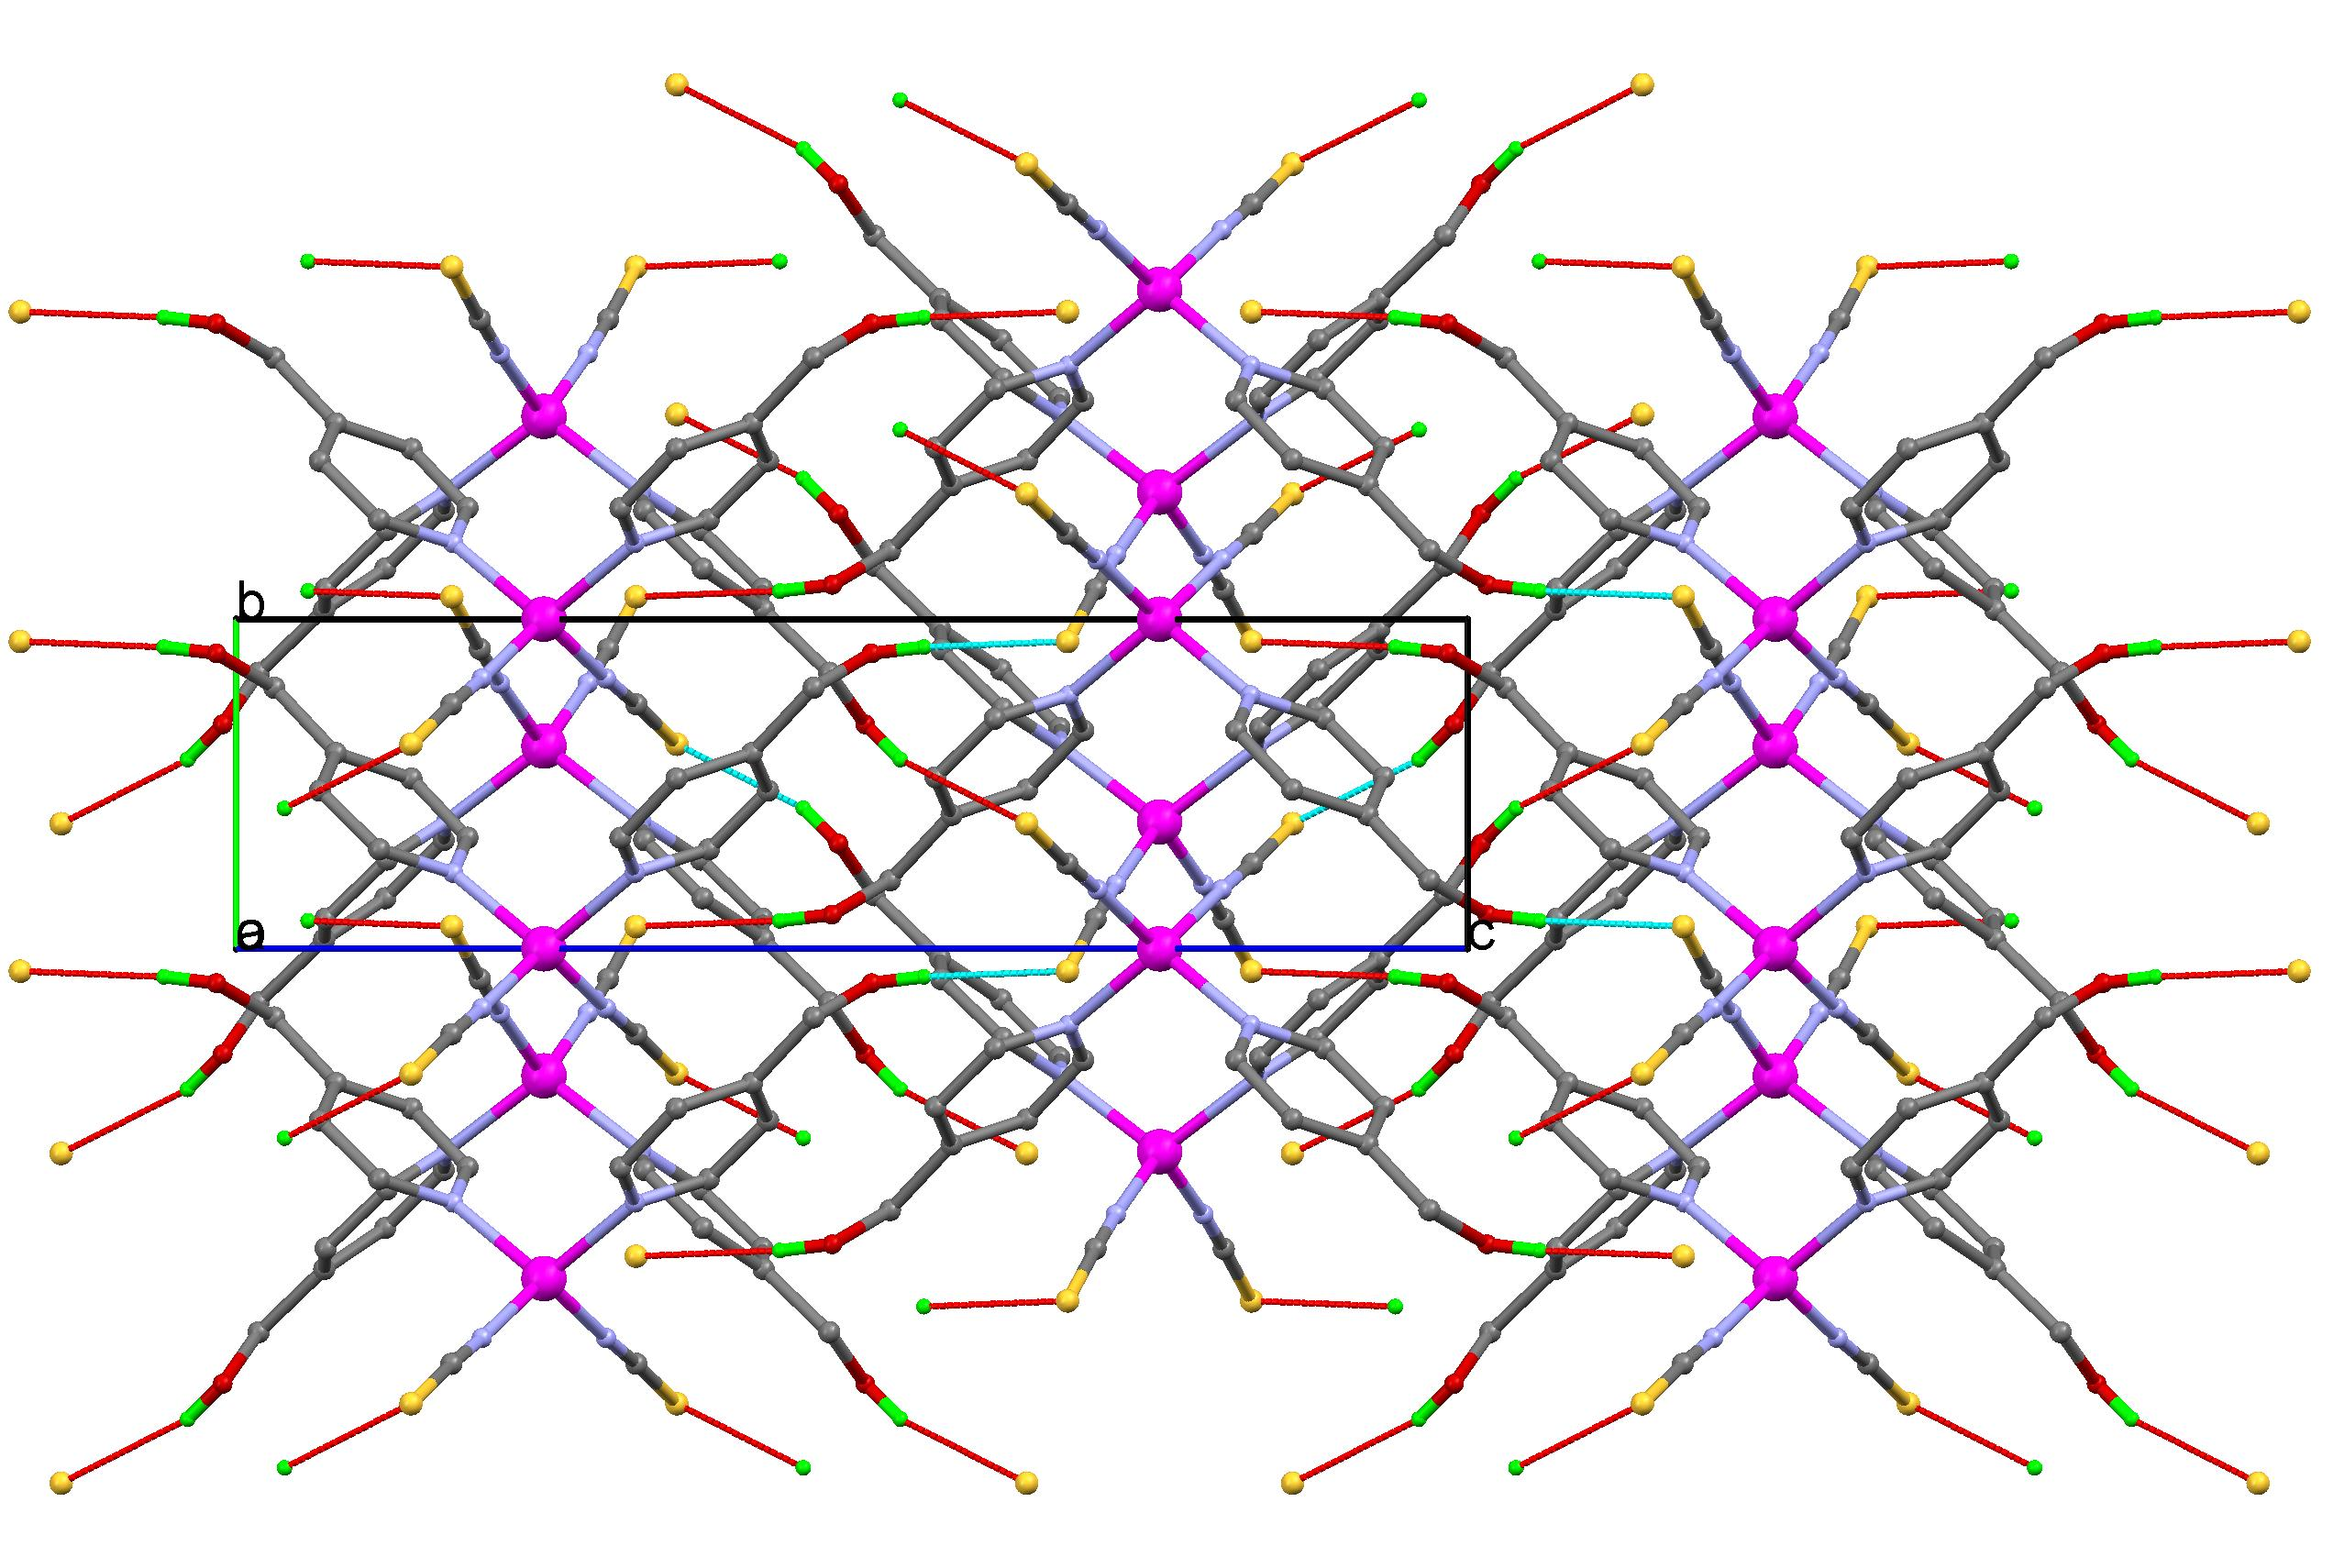
\includegraphics[width=1\textwidth]{figures/znr_4omp_CA.png}
\caption{Packing view of \ce{[Zn(SCN)_2(4-HOMepy)_2]}}
\label{fig:ZnR4HOMP_packv}
\end{figure}

\renewcommand{\arraystretch}{1.5}
\begin{table}
\centering
\captionabove{Crystallographic data and processing parameter of \ce{[Zn(SCN)_2(4-HOMepy)_2]}}
\begin{tabular}{ | l |  l | }
\hline
Empirical formula & \ce{C_{14}H_{14}N_{4}O_{2}S_{2}Zn}\\
\hline
Formula mass & 399.80\\
\hline
System & monoclinic\\
\hline
Space group & P2/c\\
\hline
a ({\AA}) & 18.349(2)\\
\hline
b ({\AA}) & 5.0296(7)\\
\hline
c ({\AA}) & 24.937(3)\\
\hline
$\alpha$ ($^\circ$) & 90\\
\hline
$\beta$ ($^\circ$) & 161.136(4)\\
\hline
$\gamma$ ($^\circ$) & 90\\
\hline
V (\AA$^{3}) $  & 1733.3(4)\\
\hline
Z & 4\\
\hline
T (K) & 100(2)\\
\hline
$\mu$ (mm$^{-1}$) & 1.670\\
\hline
 D$_{calc}$ (Mg/m$^{3}$) & 1.532\\
\hline
Crystal size (mm) & 0.27 x 0.19 x 0.11\\
\hline
$\theta$ max ($^\circ$) & 26.33\\
\hline
Data collected & 12908\\
\hline
Unique refl./ R$_{int}$ & 3529 / 0.0403\\
\hline
Parameters & 215\\
\hline
Goodness-of-Fit on F$^{2}$ & 1.112\\
\hline
R1 / wR2 (all data) & 0.0429 /0.0973\\
\hline
Residual extrema (e/\AA$^{3}$) & 0.84 /-0.44\\
\hline
\end{tabular}
\label{tab:ZnR4HOMP}


\end{table}



